\documentclass[landscape,footrule]{foils}
\usepackage[lecture-serie]{foiltex-extra}
\usepackage{color}
\usepackage{crysymb}
\usepackage[draft]{crygame}
\usepackage{crypto-ii}
\usepackage{graphics}
\usepackage[pdftex]{graphicx} 


\newcommand{\lecture}{Zero-knowledge Proofs}
\newcommand{\lserie}{MTAT.07.003 Cryptology II}
\newcommand{\ldate}{18 November, 2021}
\newcommand{\lauthor}{Sven Laur}
\newcommand{\linst}{University of Tartu}
\graphicspath{{./illustrations/}}


\newcommand{\probes}{\mathsf{probes}}
\newcommand{\lastline}{\vspace*{-2ex}}
\newcommand{\spreadappart}{\vspace*{\fill}}


\renewcommand{\SK}{{\red{\mathsf{sk}}}}
\renewcommand{\PK}{{\blue{\mathsf{pk}}}}




\begin{document}
\titlefoil



\middlefoil{Formal Syntax}
\LogoOn


\foilhead[-2cm]{Zero-knowledge proofs}

\illustration[scale=0.75, angle=-90, clip, trim=1.5cm 0.0cm 12.0cm 0.0cm]{zero-knowledge-proof.eps}

In many settings, some system-wide or otherwise important
parameters $\PK$ are generated by potentially malicious participants.
\begin{triangles}
\item Zero-knowledge proofs guarantee that the parameters $\PK$ are
  correctly generated without leaking any extra information.
\item Often, public parameters $\PK$ are generated together with
  auxiliary secret information $\SK$ that is essential for the
  zero-knowledge proof.
\item The secret auxiliary information $\SK$ is known as a
  \emph{witness} of $\PK$.
\end{triangles}

\foilhead[-1cm]{A few interesting statements}

\underline{\smash{An integer $n$ is a RSA modulus}}: 
\begin{triangles}
  \item A witness is a pair of primes $(p,q)$ such that $n=p\cdot q$.
  \item The relation is defined as follows $(n,p,q)\in R\Leftrightarrow n=p\cdot q\wedge p,q\in\PP$
\end{triangles}\vspace*{3ex}

\underline{\smash{A prover has a secret key $\SK$ that corresponds to a public key $\PK$}}:
\begin{triangles}
  \item A witness is a secret key $\SK$ such that $(\PK,\SK)\in\GEN$.
  \item More formally $(\PK,\SK)\in R\Leftrightarrow\forall m\in\MSPACE:\DEC_\SK(\ENC_\PK(m))=m$.
\end{triangles}\vspace*{3ex}
 
\underline{\smash{A ciphertext $c$ is an encryption of $m$ wrt the public key $\PK$}}:
\begin{triangles}
  \item A witness is a randomness $r\in\RSPACE$ such that $\ENC_\PK(m;r)=c$.
  \item The relation is defined as follows $(\PK,c,m,r)\in R\Leftrightarrow \ENC_\PK(m;r)=c$.
\end{triangles}\vspace*{3ex}


\foilhead[-1cm]{Two flavours of zero knowledge}\enlargethispage{1cm}

\illustration[scale=0.80, angle=-90, clip, trim=2.5cm 0.0cm 3.0cm 0.0cm]{ideal-implementation}

\foilhead[-1cm]{Formal security requirements}

\textbf{Completeness.} A zero-knowledge proof is \emph{perfectly
  complete} if all runs between honest prover and honest verifier are
accepting. A zero knowledge protocol is
$\varepsilon_1$-\emph{incomplete} if for all $(\PK,\SK)\in R$ the
interaction between honest prover and honest verifier fails with
probability at most $\varepsilon_1$.\vspace*{3ex}
 
\textbf{Soundness.} A zero-knowledge proof is
$\varepsilon_2$-\emph{unsound} if the probability that an honest
verifier accepts an incorrect input $\PK$ with probability at most
$\varepsilon_2$. An input $\PK$ is incorrect if $(\PK,\SK)\notin R$
for all possible witnesses $\SK$.\vspace*{3ex}

\textbf{Zero-knowledge property.}  A zero-knowledge proof is
$(\tre,f(\cdot),\varepsilon_3)$-\emph{private} if for any $\tre$-time
verifying strategy $\VERIFIER_*$ there exists a $f(\tre)$-time algorithm
$\VERIFIER_{\circ}$ that does not interact with the prover and the
corresponding output distributions are statistically
$\varepsilon_3$-close.\vspace*{-2ex}


\middlefoil{A Simple Example}

\foilhead[-1cm]{Quadratic residuosity}

\illustration[scale=0.75, angle=-90, clip, trim=3.5cm 0.0cm 10.0cm 0.0cm]{qr-proof}


The modified Fiat-Shamir protocol is also secure against malicious verifiers.

\begin{triangles}
\item If we guess the challenge bit $\beta$ then we can create
  $\alpha$ such that the transcript corresponds to the real world
  execution.
\item Random guessing leads to the correct answer with probability
  $\frac{1}{2}$.
\item By rewinding we can decrease the failure probability. The
  failure probability decreases exponentially w.r.t. maximal number of rewindings.
\end{triangles}

\foilhead[-1.0cm]{Simulation principle}

\illustration[scale=0.80, angle=-90, clip, trim=3.5cm 2.0cm 4.0cm 2.0cm]{simulation-principle} 

Lucy should not be able to distinguish between these two experiments.



\foilhead[-1cm]{Simulation as rejection sampling}

\begin{triangles}
\item As the Fiat-Shamir protocol is a sigma protocol, we can
  construct protocol transcripts
  $(\alpha_\circ,\beta_\circ,\gamma_\circ)\gets\SIM_{\text{Fiat\text{-}Shamir}}$ for honest
  verifier.
\item Note that $\alpha_\circ$ has the same distribution than
  $\alpha$ in the real protocol run.
\item Now consider a modified prover $\PROVER_*$ that
  \begin{diamonds}
    \item  generates $(\alpha_\circ,\beta_\circ,\gamma_\circ)\gets\SIM$ and sends $\alpha_\circ$ to the verifier,
    \item  given a challenge $\beta$ computes the correct reply $\gamma$,
    \item  outputs $\mathsf{Sim\text{-}Success}$ if $\beta_\circ=\beta$. 
  \end{diamonds}
\end{triangles}
\Bigskip

\textbf{Important observations.}  Let $\DDD_\circ$ denote the distribution
of the outputs of a verifier $\VERIFIER_*$ which satisfy the condition
$\PROVER_*$ outputs $\mathsf{Sim\text{-}Success}$. Then the
distribution $\DDD_\circ$ coincides with the distribution of all 
outputs of $\VERIFIER_*$.
\begin{triangles}
  \item For each reply $\beta$, the condition $\beta=\beta_\circ$ holds with probability $\frac{1}{2}$.
  \item The distribution $\DDD_\circ$ is easily simulatable.
\end{triangles}


\foilhead[-1cm]{The complete simulator construction}
\vspace*{-2cm}

\begin{align*}
  \begin{fblock}{\VERIFIER_\circ}
    &\!\!\begin{forblock}{i\in\set{1,\ldots,k}}
    & (\alpha_\circ,\beta_\circ,\gamma_\circ)\gets\SIM_{\text{Fiat\text{-}Shamir}}\\
    & \beta\gets\VERIFIER_*(\alpha_\circ)\\
    & \IF \beta=\beta_\circ\ \THEN \RETURN \VERIFIER_*(\gamma_\circ)\\
    \end{forblock}\\
    &\RETURN \mathsf{failure}
  \end{fblock}
\end{align*}
By the construction the output distribution of $\VERIFIER_\circ$ is
\begin{align*}
  (1-2^{-k})\DDD_\circ+2^{-k}\mathsf{failure}\equiv (1-2^{-k})\DDD+2^{-k}\mathsf{failure} 
\end{align*}
and thus the statistical distance between outputs of $\VERIFIER_*$ and
$\VERIFIER_\circ$ is $2^{-k}$.


\foilhead[-1cm]{The corresponding security guarantees}

\textbf{Theorem.} The modified Fiat-Shamir protocol is a
zero-knowledge proof with the following properties:
\begin{triangles}
  \item the protocol is perfectly complete;
  \item the protocol is $\frac{1}{2}$-unsound;
  \item for any $k$ and $\tre$ the protocol is $(\tre,k\cdot\tre,2^{-k})$-private.
\end{triangles}\vspace*{1cm}


\textbf{Further remarks}
\begin{triangles}
\item Sequential composition of $\ell$ protocol instances decreases
  soundness error to $2^{-\ell}$. The compound protocol becomes
  $(\tre,k\cdot\ell\cdot\tre,\ell\cdot 2^{-k})$-private.
\item The same proof is valid for all sigma protocols, where the
  challenge $\beta$ is only one bit long. For longer challenges
  $\beta$, the success probability decreases with an exponential rate
  and simulation becomes inefficient.
\end{triangles}

\middlefoil{Zero-Knowledge Proofs \\ and\vspace*{1ex} \\ Knowledge Extraction}


\foilhead[-1cm]{Challenge-response paradigm}

\illustration[scale=0.75, angle=-90, clip, trim=3.5cm 0.0cm 11.0cm 0.0cm]{qnr-proof-i}


For semi-honest provers it is trivial to simulate the interaction,
since the verifier knows the expected answer
$\beta=\overline{\beta}$. To provide security against malicious
verifiers $\VERIFIER_*$, we must assure that we can extract
$\beta$ from $\VERIFIER_*$:
\begin{triangles}
  \item Verifier must prove that she knows $(r,\beta)$ such that $c=r^2v^{\beta}$ 
  \item The corresponding proof of knowledge does not have be zero
    knowledge proof as long as it does not decrease soundness.
\end{triangles}

\foilhead[-1cm]{Classical construction}

\illustration[scale=0.75, angle=-90, clip, trim=3.5cm 0.0cm 11.0cm 0.0cm] {qnr-proof-iii}

We can use proofs of knowledge to assure that the verifier knows the
end result $\beta$. The proof must perfectly hide  information about witness
$\beta$.
\begin{triangles}
\item If $v\in\mathsf{QR}$ then $\alpha$ is independent from $\beta$
  and malicious prover can infer information about $\beta$ only
  through the proof of knowledge.
\item Hence, we are interested in \emph{witness indistinguishability}
  of the proof of knowledge, i.e., the proof transcripts should
  coincide for both $\beta$ values.
\end{triangles}

\foilhead[-1cm]{Witness indistinquishability provides soundness}

We have to construct a sigma protocol for the following statement
\begin{align*}
\pok{}{\exists \beta\ \exists r: \alpha=r^2v^\beta}\equiv
\pok{}{\exists r:r^2=\alpha}\vee \pok{}{\exists r:r^2=\alpha v^{-1}}  
\end{align*}
Both sub-proofs separately can be implemented through the modified
Fiat-Shamir protocol. To achieve witness indistinguishability, we just
use disjunctive proof construction.

\begin{triangles}
\item For fixed challenge $\beta$, the sub-challenge pairs are
  uniformly chosen from a set $\BBB=\set{(\beta_1,\beta_2):
    \beta_1+\beta_2=\beta}$.

\item Hence, the interactions where $\VERIFIER$ proves
  $\pok{}{\exists r: r^2=\alpha}$ and simulates $\pok{}{\exists r:\smash{r^2=\alpha
      v^{-1}}}$ are indistinguishable form the interactions where
  $\VERIFIER$ proves $\pok{}{\exists r:\smash{r^2=\alpha v^{-1}}}$ and
  simulates $\pok{}{\exists r:\smash{r^2=\alpha}}$.
 
\item If $v=s^2$ then also $\alpha_0=r^2$ and
  $\alpha_1=r^2 v$ are indistinguishable.  
\end{triangles}
Consequently, a malicious adversary succeeds with probability
$\frac{1}{2}$ if $v=s^2$.\vspace*{-1ex}


\foilhead[-2.0cm]{Simulator construction}

\begin{align*}
  \begin{fblock}{\SSS^{\VERIFIER_*}}
    &\text{Choose randomness $\omega$ for $\VERIFIER_*$ and store $\alpha$.}\\
    &\text{Use knowledge extractor to extract $\beta$.}\\
    &\text{Run $\VERIFIER_*$ once again. }\\
    &\IF \pok{\beta}{\smash{\exists r: \alpha=r^2v^\beta}} \text{ fails} \ \THEN\\
    &\begin{cblock}
      &\text{Send $\bot$ to $\VERIFIER$ and output whatever $\VERIFIER_*$ outputs.}       
    \end{cblock}\\
    &\ELSE\\
    &\begin{cblock}
      &\text{Send $\beta$ to $\VERIFIER$ and output whatever $\VERIFIER_*$ outputs.}       
     \end{cblock}\\
  \end{fblock}
\end{align*}
The simulation fails only if knowledge extraction fails and
$\pok{\beta}{\cdot}$ succeeds. With proper parameter choice, we can
achieve failure $\varepsilon$ in time $\Theta\bigl(\frac{\tre}{\varepsilon-\kappa}\bigr)$.\vspace*{-2ex}


\foilhead[-1.0cm]{Optimal choice of parameters}

Let $\varepsilon$ be the desired failure bound and let $\kappa$ be the
knowledge error of the sigma protocol. Now if we set the maximal
number of repetitions
\begin{align*}
  \ell=\frac{4\ceil{\log_2(1/\varepsilon)}}{\varepsilon-\kappa}
\end{align*}
in the knowledge extraction algorithm so that the knowledge extraction
procedure fails on the set of good coins
\begin{align*}
  \Omega_{\mathrm{good}}=\set{\omega\in\Omega:\pr{\pok{\beta}{\cdot}=1|\omega}\geq \varepsilon}
\end{align*}
with probability less than $\varepsilon$. Consequently, we can estimate
    \begin{align*}
      \pr{\mathsf{Fail}}%
      &\leq\pr{\omega\notin\Omega_{\mathrm{good}}}\cdot\pr{\pok{\beta}{\cdot}=1|\omega}
      \cdot \pr{\mathsf{ExtrFailure}|\omega}\\
      &\quad+\pr{\omega\in\Omega_{\mathrm{good}}}\cdot\pr{\pok{\beta}{\cdot}=1|\omega}\cdot
      \pr{\mathsf{ExtrFailure}|\omega}\leq\varepsilon\enspace.
    \end{align*}\ \vspace*{-8ex}\\



\foilhead[-1cm]{Soundness through temporal order}

\illustration[scale=0.75, angle=-90, clip, trim=3.5cm  0.0cm 11.0cm 0.0cm] {qnr-proof-ii}

Let $(\GEN,\COM,\OPEN)$ is a perfectly binding commitment
scheme such that the validity of public parameters can be verified
(ElGamal encryption).
\begin{triangles}
\item Then the perfect binding property assures that the malicious
  prover $\PROVER_*$ cannot change his reply. Soundness guarantees are
  preserved.
\item A commitment scheme must be $(\tre+t,\kappa)$-hiding for $\tre$-time verifier.
\item By rewinding we can find out the correct answer in time
  $\Theta(\frac{1}{\varepsilon-\kappa})$, where $\varepsilon$ is the
  success probability of malicious verifier $\VERIFIER_*$.
\end{triangles}

\foilhead[-3.0cm]{Simulator construction} 
\begin{align*}
  \begin{fblock}{\SSS^{\VERIFIER_*}}
    &\text{Choose randomness $\omega$ for $\VERIFIER_*$ and store $\alpha$.}\\
    &\text{Use knowledge extractor to extract $\beta$.}\\
    &\text{Run $\VERIFIER_*$ once again with $(c,d)\gets\COM_\PK(\beta)$.}\\
    &\IF \alpha\neq r^2v^\beta  \ \THEN\\
    &\begin{cblock}
      &\text{Send $\bot$ to $\VERIFIER$ and output whatever $\VERIFIER_*$ outputs.}       
    \end{cblock}\\
    &\ELSE\\
    &\begin{cblock}
      &\text{Send $d$ to $\VERIFIER$ and output whatever $\VERIFIER_*$ outputs.}       
     \end{cblock}\\
  \end{fblock}
\end{align*}
Knowledge-extraction is straightforward. We just provide
$(c,d)\gets\COM_\PK(0)$ and verify whether $\alpha=r^2v^\beta$. The
choice of parameters is analogous.\vspace*{-2ex} 

\foilhead[-1.5cm]{Further analysis} 

The output of the simulator is only computationally indistinguishable
from the real protocol run, as the commitment is only computationally hiding.
Let $\AD$ be a $t$-time adversary that tries to distinguish outputs of
$\VERIFIER_*$ and $\SSS^{\VERIFIER_*}$

\begin{triangles}
\item  If $\alpha=r^2v^\beta$ and knowledge
  extraction succeeds,  the simulation is perfect.
\item If $\alpha\neq r^2v^{\beta}$ then from $(\tre+t,\kappa)$-hiding, we get
    \begin{align*}
      \abs{\pr{\AD=1|\VERIFIER_*^\PROVER\wedge\alpha\neq r^2v^{\beta}}
           -\pr{\AD=1|\SSS^{\VERIFIER_*}\wedge\alpha\neq r^2v^{\beta}}}\leq \kappa\enspace.
    \end{align*}
\item Similarly, $(\tre+t,\kappa)$-hiding assures that
    \begin{align*}
      \abs{\pr{\alpha=r^2v^{\beta}|\VERIFIER_*^\PROVER}
           -\pr{\alpha\neq r^2v^{\beta}|\VERIFIER_* \wedge (c,d)\gets\COM_\PK(0)}}\leq \kappa\enspace.
    \end{align*}
    Hence, the knowledge extractor makes on average $\frac{1}{\varepsilon-\kappa}$ probes. 
\end{triangles}


\middlefoil{Strengthening of $\Sigma$-protocols}

\foilhead[-1.5cm]{Strengthening with commitments}

\illustration[scale=0.75, angle=-90, clip, trim=1.5cm
  0.0cm 11.0cm 0.0cm]{strengthened-sigma-proof-i}

If the commitment is statistically hiding then the soundness
guarantees are preserved. Again, rewinding allows us to extract the
value of $\beta$.
\begin{triangles}
\item If commitment scheme is
  $((\ell+1)\cdot\tre,\varepsilon_2)$-binding then commitment can be
  double opened with probability at most $\varepsilon_2$.
\item Hence, we can choose $\ell=\Theta(\frac{1}{\varepsilon_1})$ so
  that simulation failure is $\varepsilon_1+\varepsilon_2$.
\item The protocol does not have knowledge extraction property any more.
\end{triangles}

\foilhead[-1.5cm]{Strengthening with coin-flipping}

\illustration[scale=0.75, angle=-90, clip, trim=1.5cm 0.0cm 11.0cm 0.0cm]{strengthened-sigma-proof-ii}

We can substitute trusted sampling $\beta\getsu\BBB$ with a
coin-flipping protocol.

\begin{triangles}
\item To achieve soundness, we need a coin-flipping protocol that is
  secure against unbounded provers.
\item Statistical indistinguishability is achievable provided that the
  coin-flipping protocol is secure even if all internal variables
  become public afterwards.
\item Rewinding takes now place inside the coin-flipping block.
\end{triangles}

\foilhead[-1.5cm]{Strengthening with disjunctive proofs}

\illustration[scale=0.75, angle=-90, clip, trim=1.5cm 0.0cm 11.0cm 0.0cm]{strengthened-sigma-proof-iii}

If the relation $\overline{R}$ generated by $\GEN_{\overline{R}}$ is
hard, i.e., given $\overline{x}$ it is difficult to find matching
$\overline{w}$, then the proof is computationally sound.

The hardness of $\overline{R}$ also guarantees that the second proof
is witness hiding. Thus, we can extract first $\overline{w}$ and use
it to by-pass the second proof.


\middlefoil{Certified Computations\vspace*{1ex}\\{\normalsize Malicious case}}

\foilhead[-1cm]{The concept}\enlargethispage{1cm}

\illustration[scale=0.80, angle=-90, clip, trim=3.5cm 0.0cm 3.5cm 0.0cm]{certified-computations}
Lucy should learn $f(x)$ and nothing more even if Charlie is malicious.



\foilhead[-1cm]{A quick recap of the semihonest case}\enlargethispage{1cm}

\begin{center}
\begin{tabular}{|c|}
 \hline
 Construct the circuit and commit all values\\
  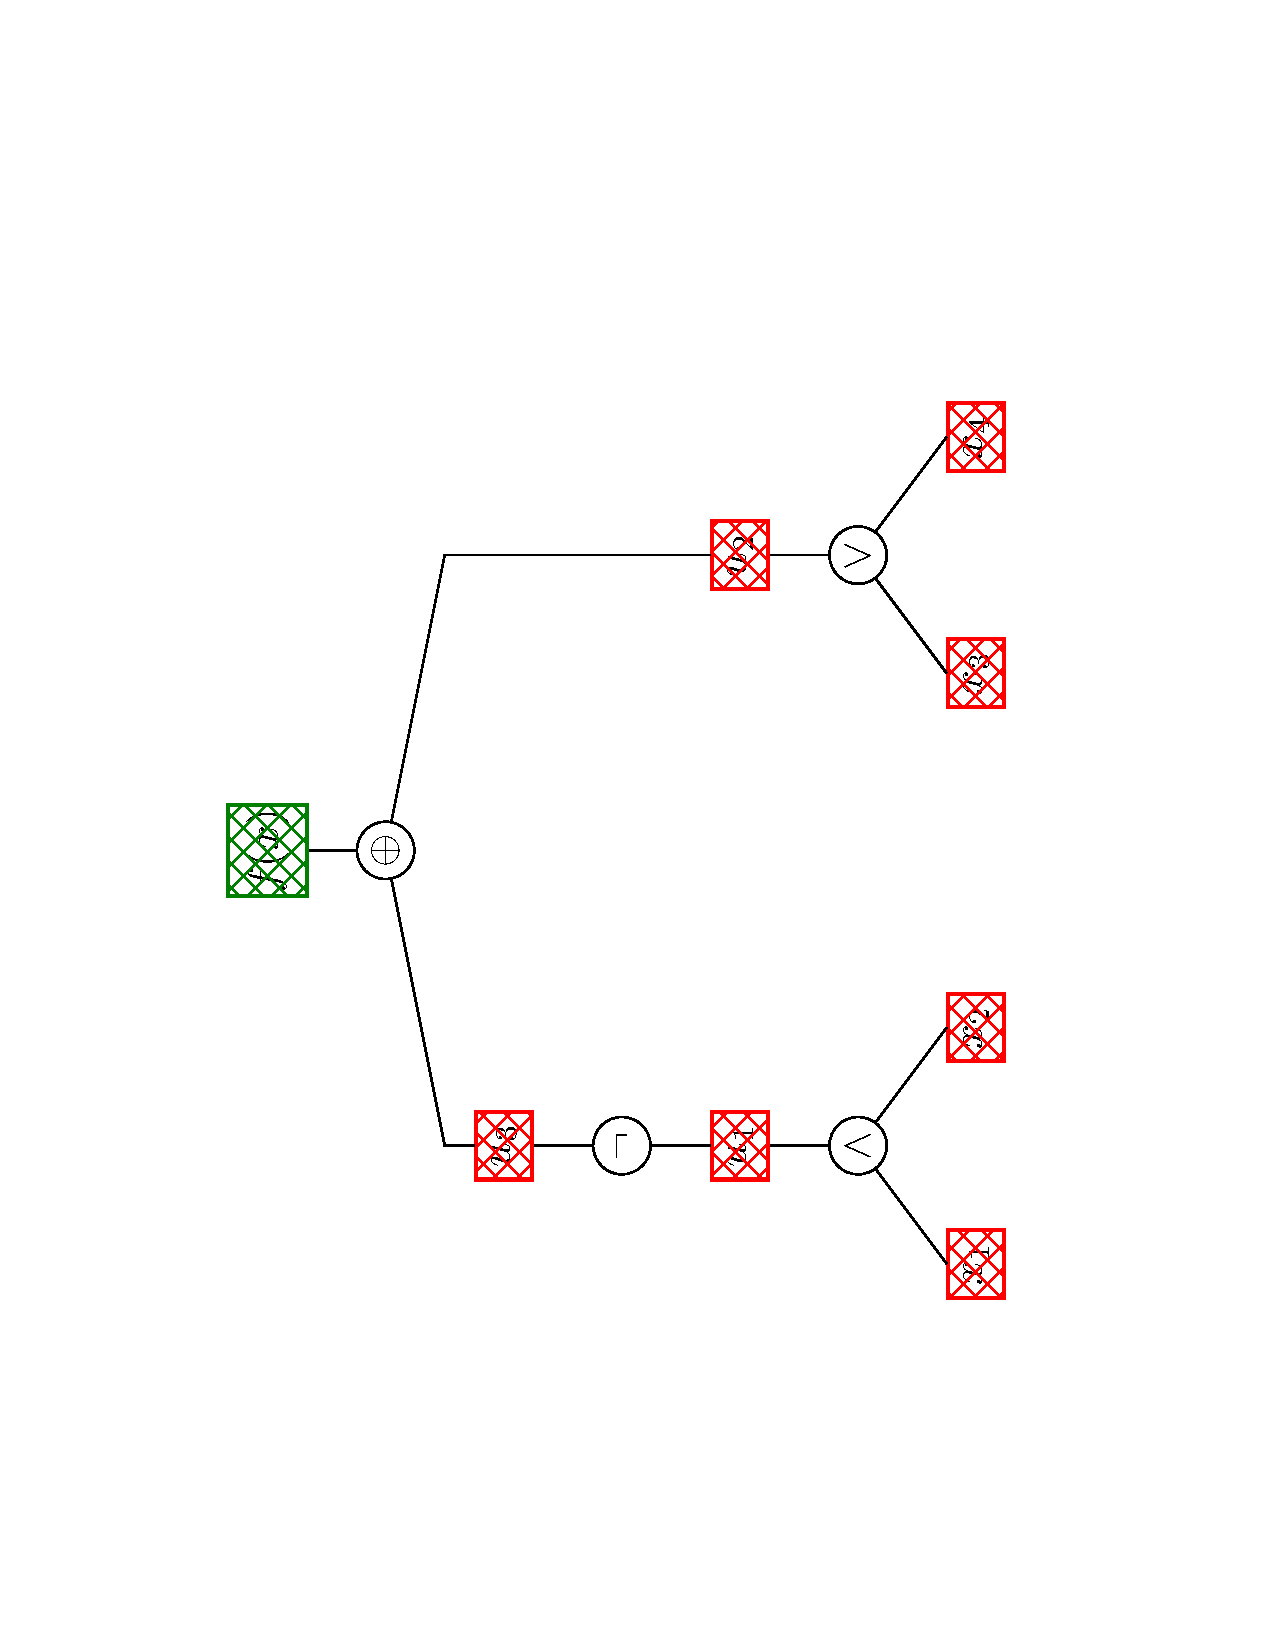
\includegraphics[scale=0.18, angle=-90, clip, trim=3.5cm 0.0cm 3.5cm 0.0cm]{boolean-circuit}\\  
\hline
 Construct a sigma protocols for validity of inputs\\
 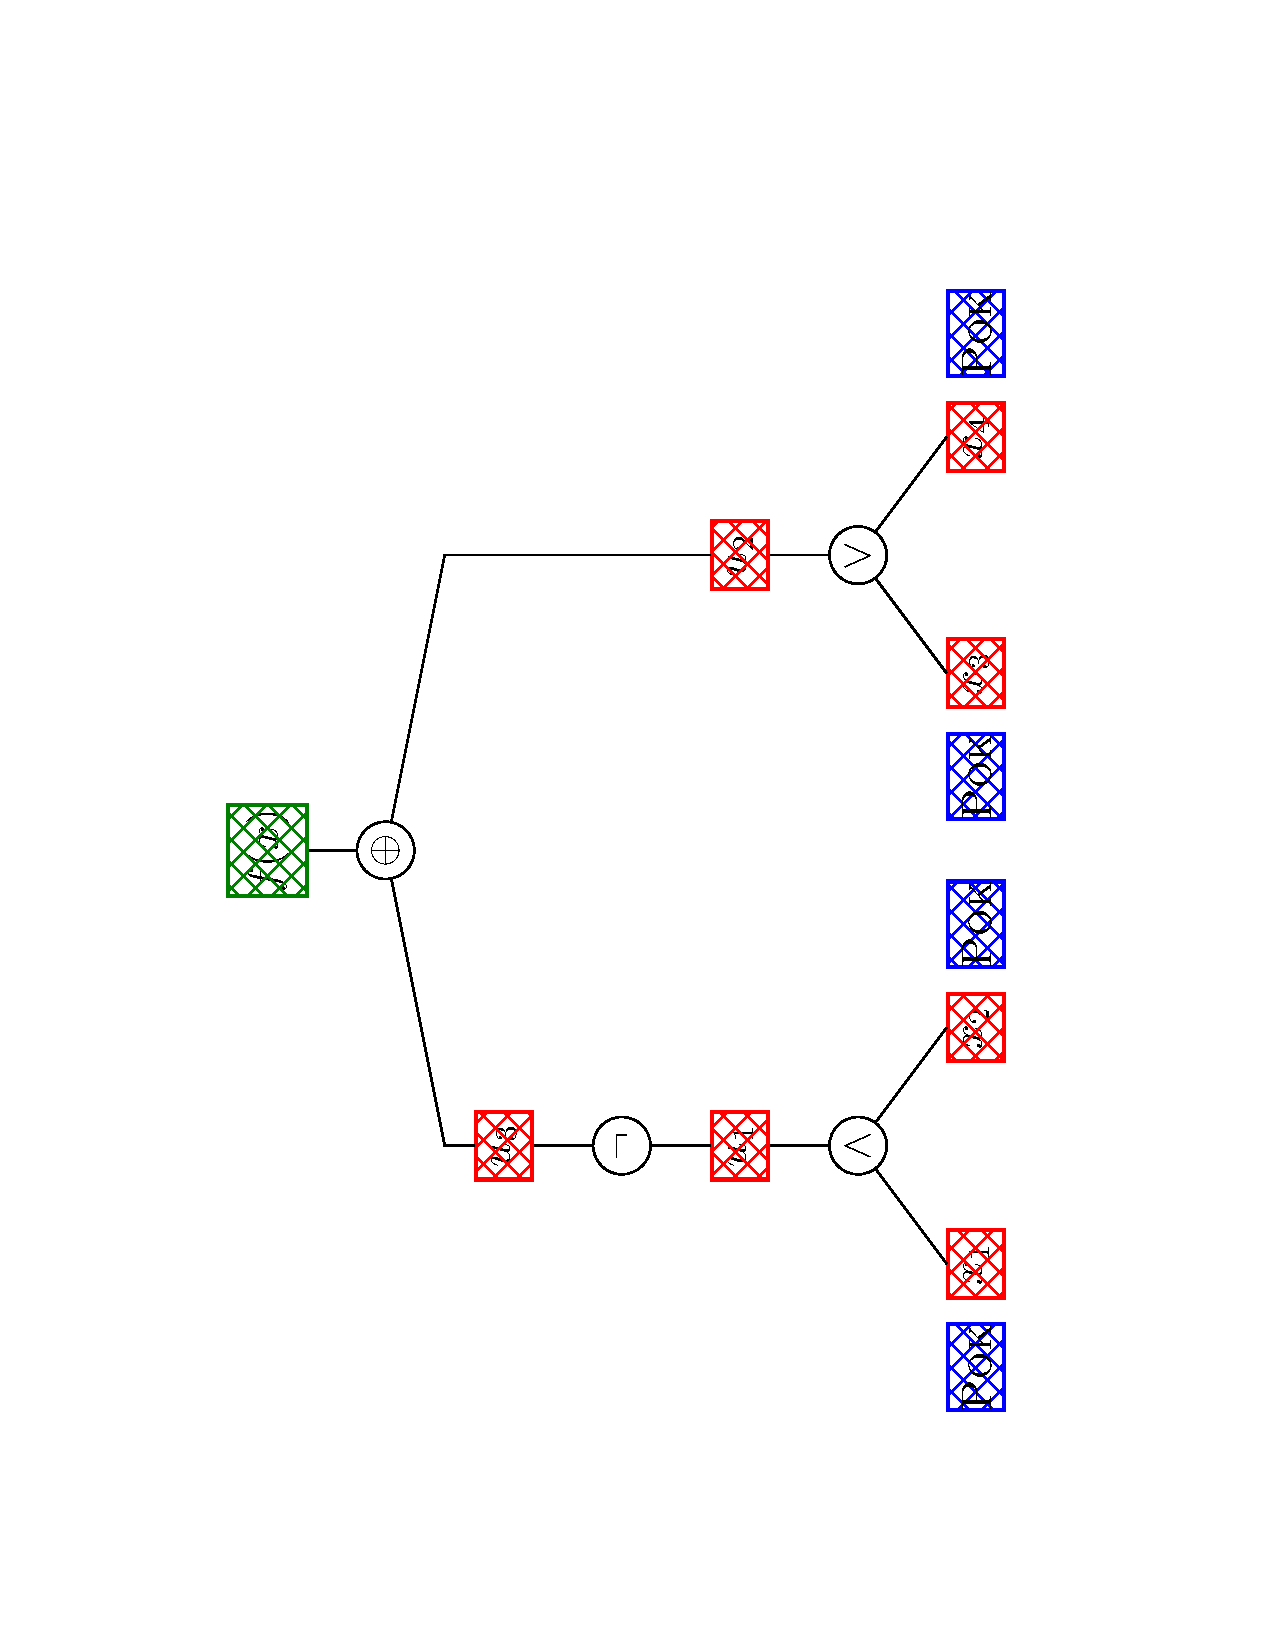
\includegraphics[scale=0.18, angle=-90, clip, trim=3.0cm 0.0cm 3.5cm 0.0cm]{augmented-circuit-i}\\
\hline
 Construct a sigma protocol for validity of intermediate values\\ 
  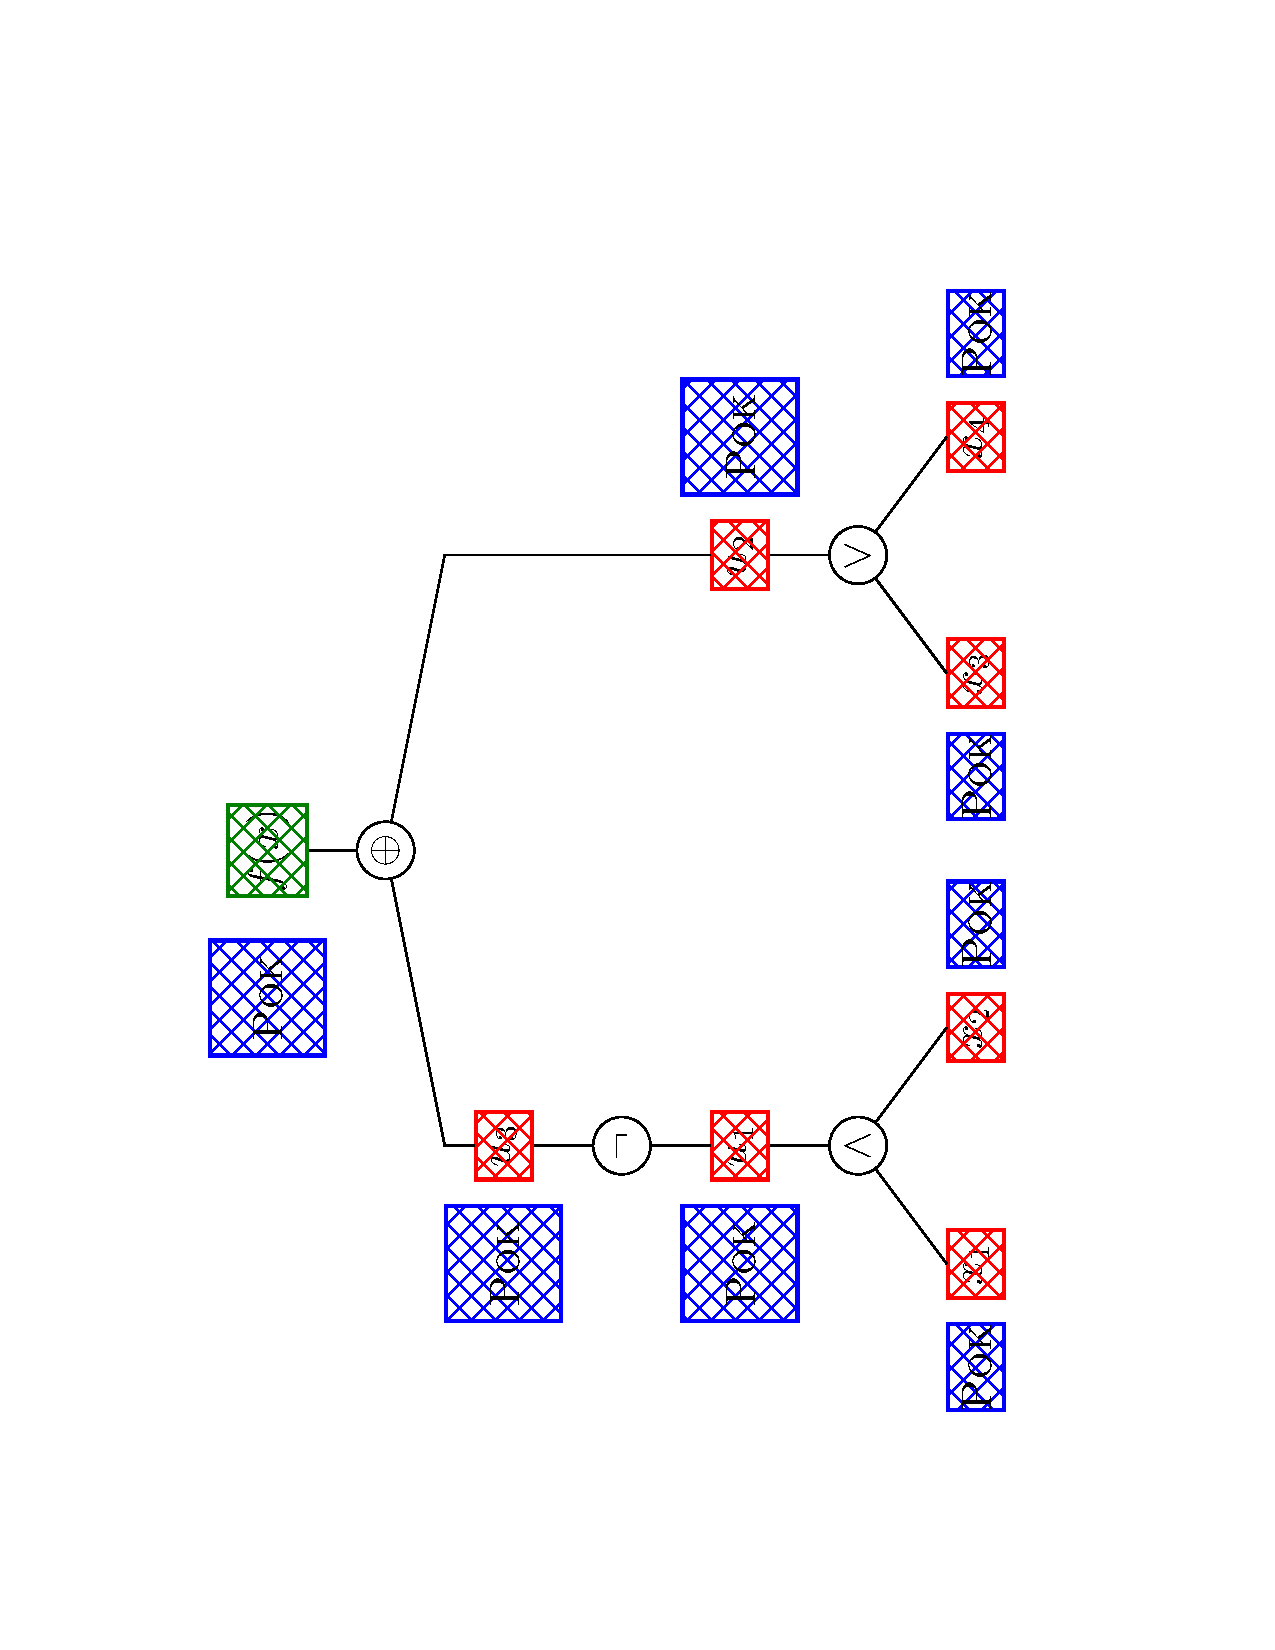
\includegraphics[scale=0.18, angle=-90, clip, trim=3.0cm 0.0cm 3.5cm 0.0cm]{augmented-circuit-ii}\\
\hline
\end{tabular}
\end{center}

\foilhead[-1cm]{Security against malicious verifiers}

We can use several methods to strengthen the protocol. 
\begin{triangles}
\item We can restrict challenge space $\BBB$ to $\set{0,1}$ and then
  use sequential composition to achieve reasonable soundness level.
\item We can use commitments to strengthen the sigma protocol.
\item We can use coin-flipping protocol to generate the challenge $\beta$.
\item We can use disjunctive proofs to strengthen the sigma protocol.
\end{triangles}
\Bigskip

The resulting construction which is based on a coin-flipping protocol
is often referred as $\textsc{Gmw}$-compiler, since it forces
semihonest behaviour.


\end{document}


